% ------------------------------------------------------------------
\documentclass[12 pt]{article} % A4 paper set by geometry package below
\pagenumbering{arabic}
\setlength{\parindent}{10 mm}
\setlength{\parskip}{12 pt}

% Nimbus Sans font should be reasonably legible
\usepackage{helvet}
\renewcommand{\familydefault}{\sfdefault}
\usepackage[T1]{fontenc}  % Without this \textsterling produces $

% Section header spacing
\usepackage{titlesec}
\titlespacing\section{0pt}{12pt plus 4pt minus 2pt}{0pt plus 2pt minus 2pt}
\titlespacing\subsection{0pt}{12pt plus 4pt minus 2pt}{0pt plus 2pt minus 2pt}
\titlespacing\subsubsection{0pt}{12pt plus 4pt minus 2pt}{0pt plus 2pt minus 2pt}

\usepackage{amsmath}
\usepackage{amssymb}
\usepackage{graphicx}
\usepackage{verbatim}    % For comment
\usepackage[paper=a4paper, marginparwidth=0 cm, marginparsep=0 cm, top=2.5 cm, bottom=2.5 cm, left=3 cm, right=3 cm, includemp]{geometry}
\usepackage[pdftex, pdfstartview={FitH}, pdfnewwindow=true, colorlinks=true, citecolor=blue, filecolor=blue, linkcolor=blue, urlcolor=blue, pdfpagemode=UseNone]{hyperref}

% Put module code and last-modified date in footer
\usepackage{fancyhdr}
\pagestyle{fancy}
\fancyhf{}
\renewcommand{\headrulewidth}{0pt}
\cfoot{{\small \thisunit}\hfill \thepage\hfill {\small \moddate}}

% Hopefully address Canvas complaints about pdf tagging
%\usepackage[tagged]{accessibility}
\hypersetup {
  pdfauthor={David Schaich},
  pdftitle={Statistical Physics Tutorial Activity},
}
% ------------------------------------------------------------------



% ------------------------------------------------------------------
% Shortcuts
\newcommand{\cO}{\ensuremath{\mathcal O} }
\newcommand{\al}{\ensuremath{\alpha} }
\newcommand{\be}{\ensuremath{\beta} }
\newcommand{\ga}{\ensuremath{\gamma} }
\newcommand{\eps}{\ensuremath{\varepsilon} }
\newcommand{\om}{\ensuremath{\omega} }
\newcommand{\Lra}{\ensuremath{\Longrightarrow} }
\newcommand{\vev}[1]{\ensuremath{\left\langle #1 \right\rangle} }
\newcommand{\pderiv}[2]{\ensuremath{\frac{\partial #1}{\partial #2}} }
% ------------------------------------------------------------------



% ------------------------------------------------------------------
\begin{document}
\newcommand{\thisunit}{MATH327 Tutorial (Debye)}
\newcommand{\moddate}{Last modified 25 Apr.~2024}
\begin{center}
  {\Large \textbf{MATH327: Statistical Physics, Spring 2024}} \\[12 pt]
  {\Large \textbf{Tutorial activity \ --- \ Debye solid}} \\[24 pt]
\end{center}

This activity will be introduced in our 25 April tutorial, and you'll have until our next tutorial on 2 May to work on it.
In particular, in the next lecture we'll discuss the non-relativistic fermion gas needed for the second task below.
You already have everything you need to solve the first task adapting the photon gas.

We have seen that Einstein's simple non-interacting model of a solid predicts the heat capacity
\begin{equation*}
  c_v = N \left(\frac{\hbar \om}{T}\right)^2 \frac{e^{\hbar \om / T}}{\left(e^{\hbar \om / T} - 1\right)^2} = \frac{N x^2 e^x}{\left(e^x - 1\right)^2},
\end{equation*}
with $x \equiv \be\hbar\om = \hbar\om / T$.
As $T \to 0$, this vanishes exponentially rapidly,
\begin{equation*}
  \frac{c_v}{N} \approx \frac{\hbar^2 \om^2}{T^2 e^{\hbar \om / T}} \qquad \mbox{for} \qquad T \ll \hbar\om.
\end{equation*}

While the asymptotic $\lim_{T \to 0} c_v = 0$ is correct (and one way of expressing the \href{https://en.wikipedia.org/wiki/Third_law_of_thermodynamics#Specific_heat}{third law of thermodynamics}), the heat capacities of real materials vanish polynomially in $T$, as opposed to this exponential dependence.
This is demonstrated by the figure below (from Schroeder's \textit{Introduction to Thermal Physics}), which shows $c_v / T$ varying linearly with $T^2$ at low temperatures $T \lesssim 4$~K, and (for these three metals) approaching a non-zero constant value at absolute zero:
\begin{equation*}
  \frac{c_v}{T} = \al + \ga T^2 \qquad \Lra \qquad c_v = \al T + \ga T^3.
\end{equation*}

\begin{center}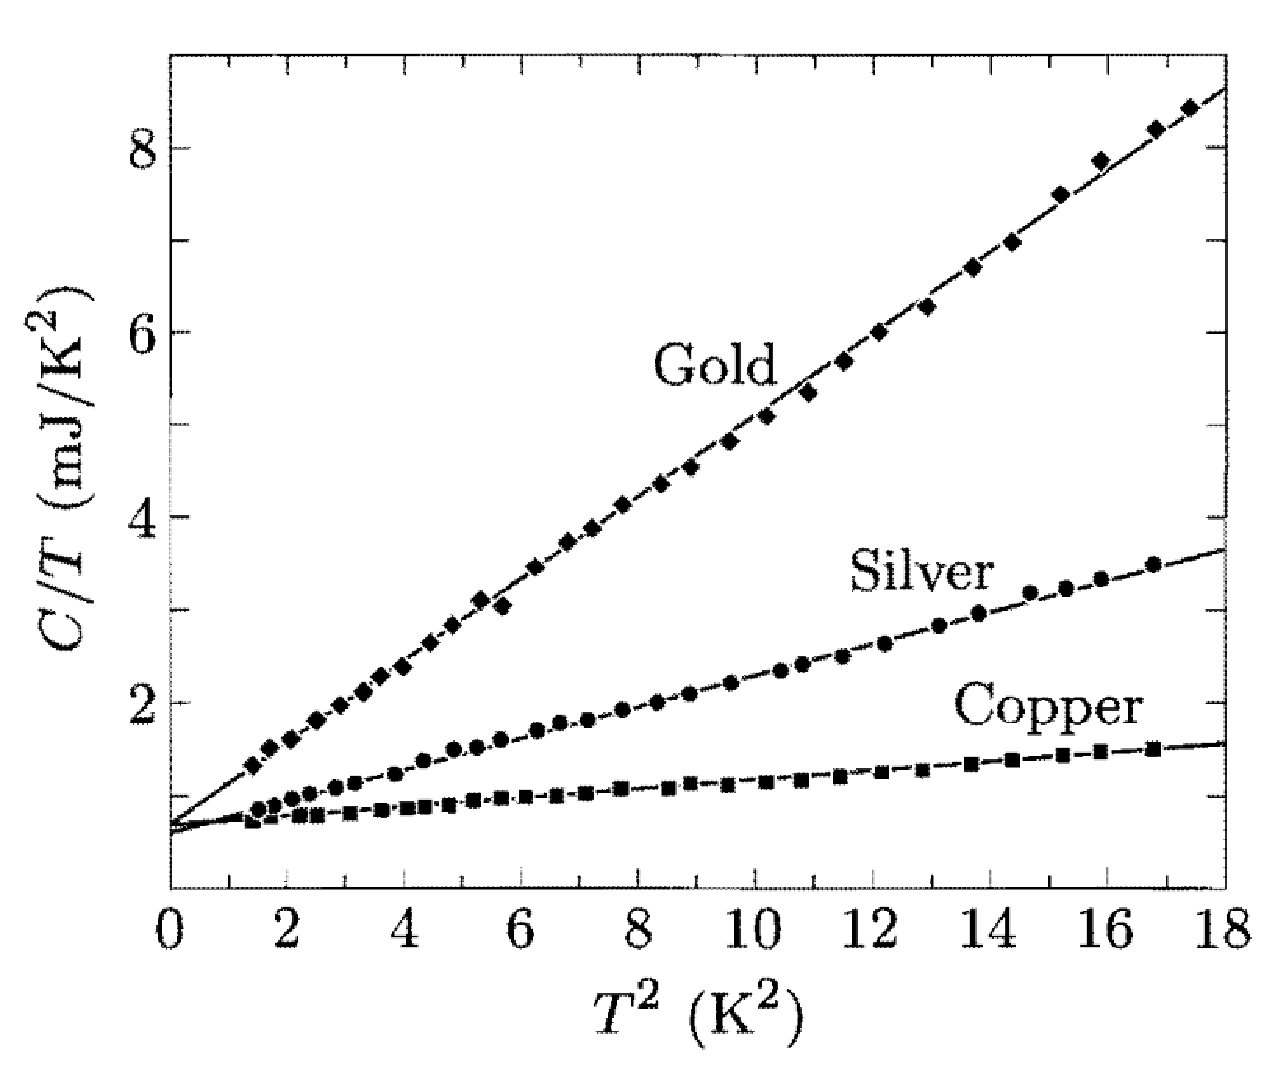
\includegraphics[width=0.7\textwidth]{figs/heat_cap-lowT.pdf}\end{center}

The two terms arise from different physical sources.
We already have the tools to analyze the $\cO(T^3)$ term, by thinking about what might be going wrong with the Einstein solid as a model of real materials.
Recall that this model treats materials as lattices of atoms that are held in place by oscillators connecting them to their nearest neighbours.
If an atom tries to move out of its position, it compresses the oscillator in the direction of its motion.
This adds (quantized) energy to the oscillator, which exerts a force to push the atom back into place.

What the Einstein solid neglects is the equal and opposite force the atom exerts on the oscillator, which the oscillator passes on to the atom on its other side.
This second atom is therefore shoved \textit{out} of place, requiring intervention from the other oscillators it's connected to.
Ultimately, we can expect this to result in patterns of correlated motion travelling long distances (relative to the atomic scale) through the solid.
Thinking of the \href{https://en.wikipedia.org/wiki/Wave_(audience)}{stadium wave} or \href{https://www.youtube.com/watch?v=uTlwzsud-zg}{plants blowing in the wind} can give us a rough mental picture of this behaviour.

Such a picture makes it clear that the Einstein-solid approach of randomly assigning units of energy to oscillators throughout the material is at best a crude approximation.
Remarkably, it is still possible to more realistically model the collective motion of many atoms in terms of non-interacting degrees of freedom.
Taking inspiration from having considered photons as quantized electromagnetic waves, we describe the propagating waves of coherent atomic motion in terms of \textbf{phonons}.\footnote{The word `phonon' (like `telephone') is based on the Greek term $\phi \om \nu o \varsigma$ (``phonos''), meaning ``sound'' --- the behaviour we have described is essentially how acoustic waves carry sound.}
Analyzing solids in terms of non-interacting phonons produces the \textbf{Debye} model (named after \href{https://en.wikipedia.org/wiki/Peter_Debye}{Peter Debye}), which provides an important foundation for modern solid-state physics.
As an aside, the concept of phonons was only introduced in 1932, about twenty years after Debye introduced his model as a refinement of the Einstein solid.
Phonons are an example of a \textit{quasi-particle} --- a collective excitation of many degrees of freedom that behaves approximately like a non-interacting particle.

\textbf{Your first task} for this activity is to determine the high- and low-temperature behaviour of the heat capacity predicted by the Debye model.
To approach this task, you can revisit the photon gas analyzed in Section~8.3 of the lecture notes, accounting for these similarities and differences between photons and phonons: \\[-24 pt]
\begin{itemize}
  \item Both photons and phonons are massless (ultra-relativistic) bosons.
  \item Phonons travel at the (material-dependent) speed of sound $c_s$ rather than at the much larger speed of light.
  \item Phonons have three polarizations compared to the photons' two, but you can feel free to neglect all numerical factors like this and consider only the functional form of the heat capacity at high and low temperatures.
  \item Most significantly, phonons possess a minimum wavelength set by the distance between the atoms in the solid, as illustrated by the figure below (also from Schroeder's \textit{Introduction to Thermal Physics}).
        This corresponds to a maximum frequency, $\om_{\text{max}} \propto \sqrt[3]{N}$ for $N$ atoms in three dimensions.
  \item While there is also a minimum frequency set by the size of the solid, even tiny solids are so large compared to the atomic scale that this minimum frequency can be set to zero.
\end{itemize}
In the end, you should find the same $T \to \infty$ limit as for the Einstein solid, while for low temperatures you should find $c_v \propto T^3 \to 0$, correcting the Einstein solid's exponential $T$-dependence.

\begin{center}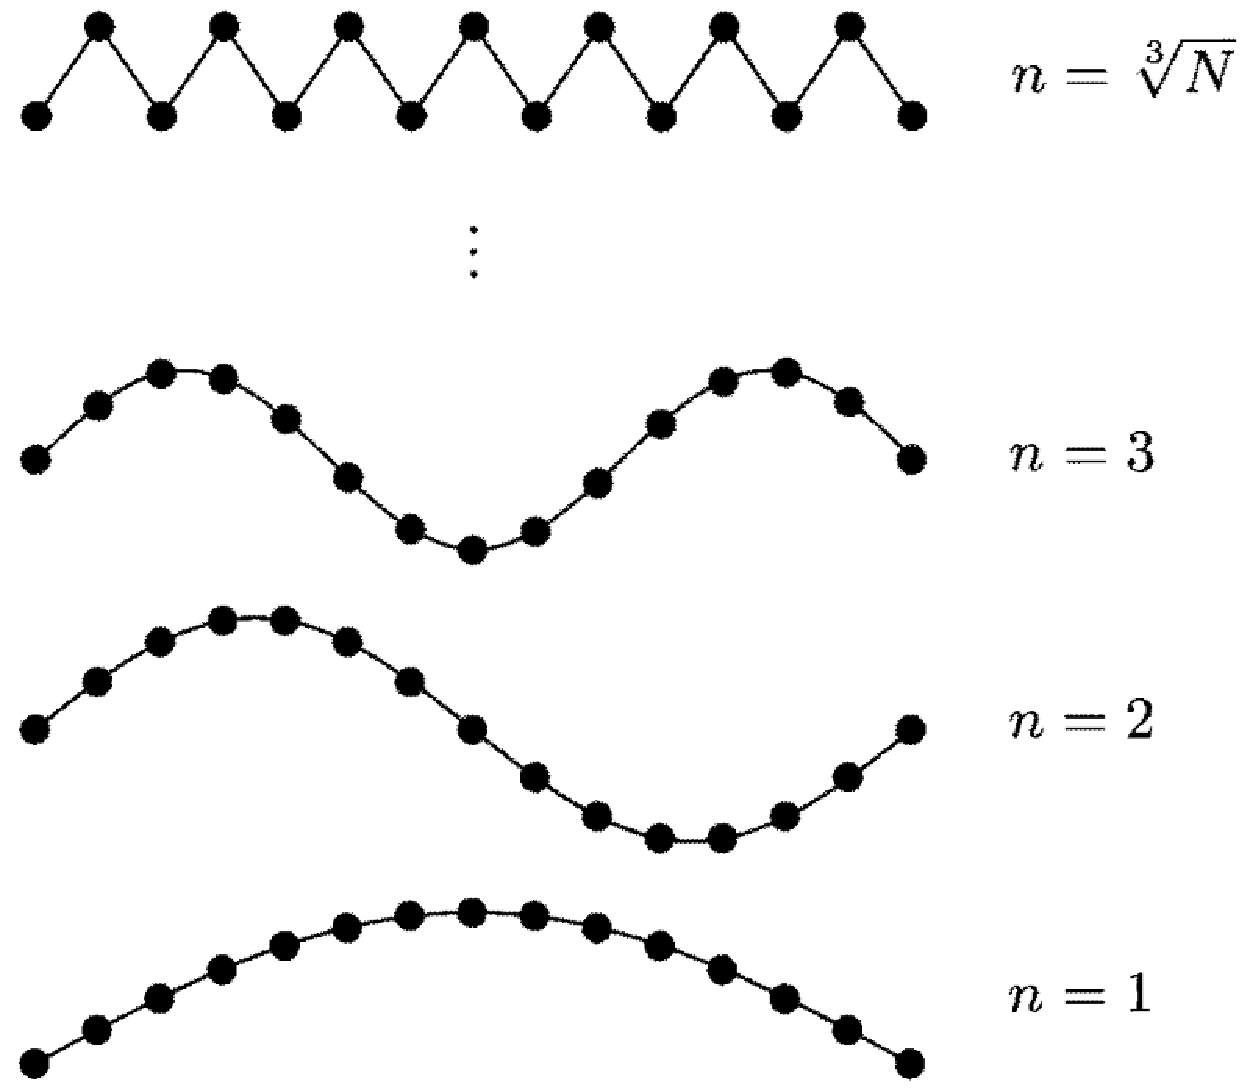
\includegraphics[width=0.6\textwidth]{figs/Debye.pdf}\end{center}

We still need to explain the origin of the linear term in the experimental data shown above.
To do so, we can note that this is most relevant at very low temperatures $\frac{T}{T_D} \ll 1 \implies \left(\frac{T}{T_D}\right)^3 \ll \frac{T}{T_D}$, where the \textit{Debye temperature} $T_D$ is here just a convenient reference scale we can use to work in terms of dimensionless numbers.
At these low temperatures, there is not enough thermal energy for any phonons to form (or oscillators to oscillate) --- the lattice of atoms is effectively frozen.
But we will soon see that ideal gases of non-relativistic fermions retain non-zero energy even as $T \to 0$.
This will provide a hint about what's going on: The linear heat capacity at very low temperatures is coming not from the atoms in the solid, but from a low-temperature gas of electrons.

\textbf{Your second task} for this activity is to determine the low-temperature behaviour of the heat capacity predicted by an ideal, non-relativistic electron gas.
This requires going beyond the approximation of the Fermi function $F(E)$ as a step function in Section~8.5 of the lecture notes.
Instead, integrate $\vev{E}_{\text{f}} \propto \int_0^{\infty} F(E) E^{3 / 2} \mathop{dE}$ by parts, then argue that the boundary term vanishes while the remaining integrand $\propto E^{5 / 2}$ is sharply peaked around $E \approx \mu$.
Expanding that $E^{5 / 2}$ factor in a Taylor series around $E = \mu$ produces simpler integrals, and by evaluating them and taking the derivative $\pderiv{}{T}\vev{E}_{\text{f}}$ you should find $c_v \propto T$ at leading order.
Again feel free to neglect numerical factors and focus on the functional form.

\end{document}
% ------------------------------------------------------------------
